\section{Relaterede undersøgelser}
\label{RelateretUndersoegelser}
%
I det følgende afsnit vil der være en kort gennemgang af tre udvalgte undersøgelser, som i en eller anden grad relaterer sig til den sideløbende opgave, der netop omhandler perifer interaktion med et musikanlæg.\blankline
%
\textcite{PDF:ComparingInputModalities} undersøger, om perifer interaktion med en musikafspiller kan lade sig gøre, når brugeren sidder foran sin computer og er igang med en primær opgave. Den perifere interaktion med musikafspilleren undersøges for tre forskellige modaliteter; et knop-baseret håndtag, en touchskærm og semaforiske gestikker, som er præsenteret på \autoref{fig:InputModalitiesMusicControl}. De semaforiske gestikker svarer i denne sammenhæng til frihåndsgetikker. Til hver af de tre modaliteter undersøger \textcite[ss. 165-166]{PDF:ComparingInputModalities} hvilken type input, der er mest fordelagtig at anvende til de mest basale funktioner, som en musikafspiller indeholder; start, pause, skift musiknummer samt justering af lydstyrken.  
%
\begin{figure}[H]
	\centering
	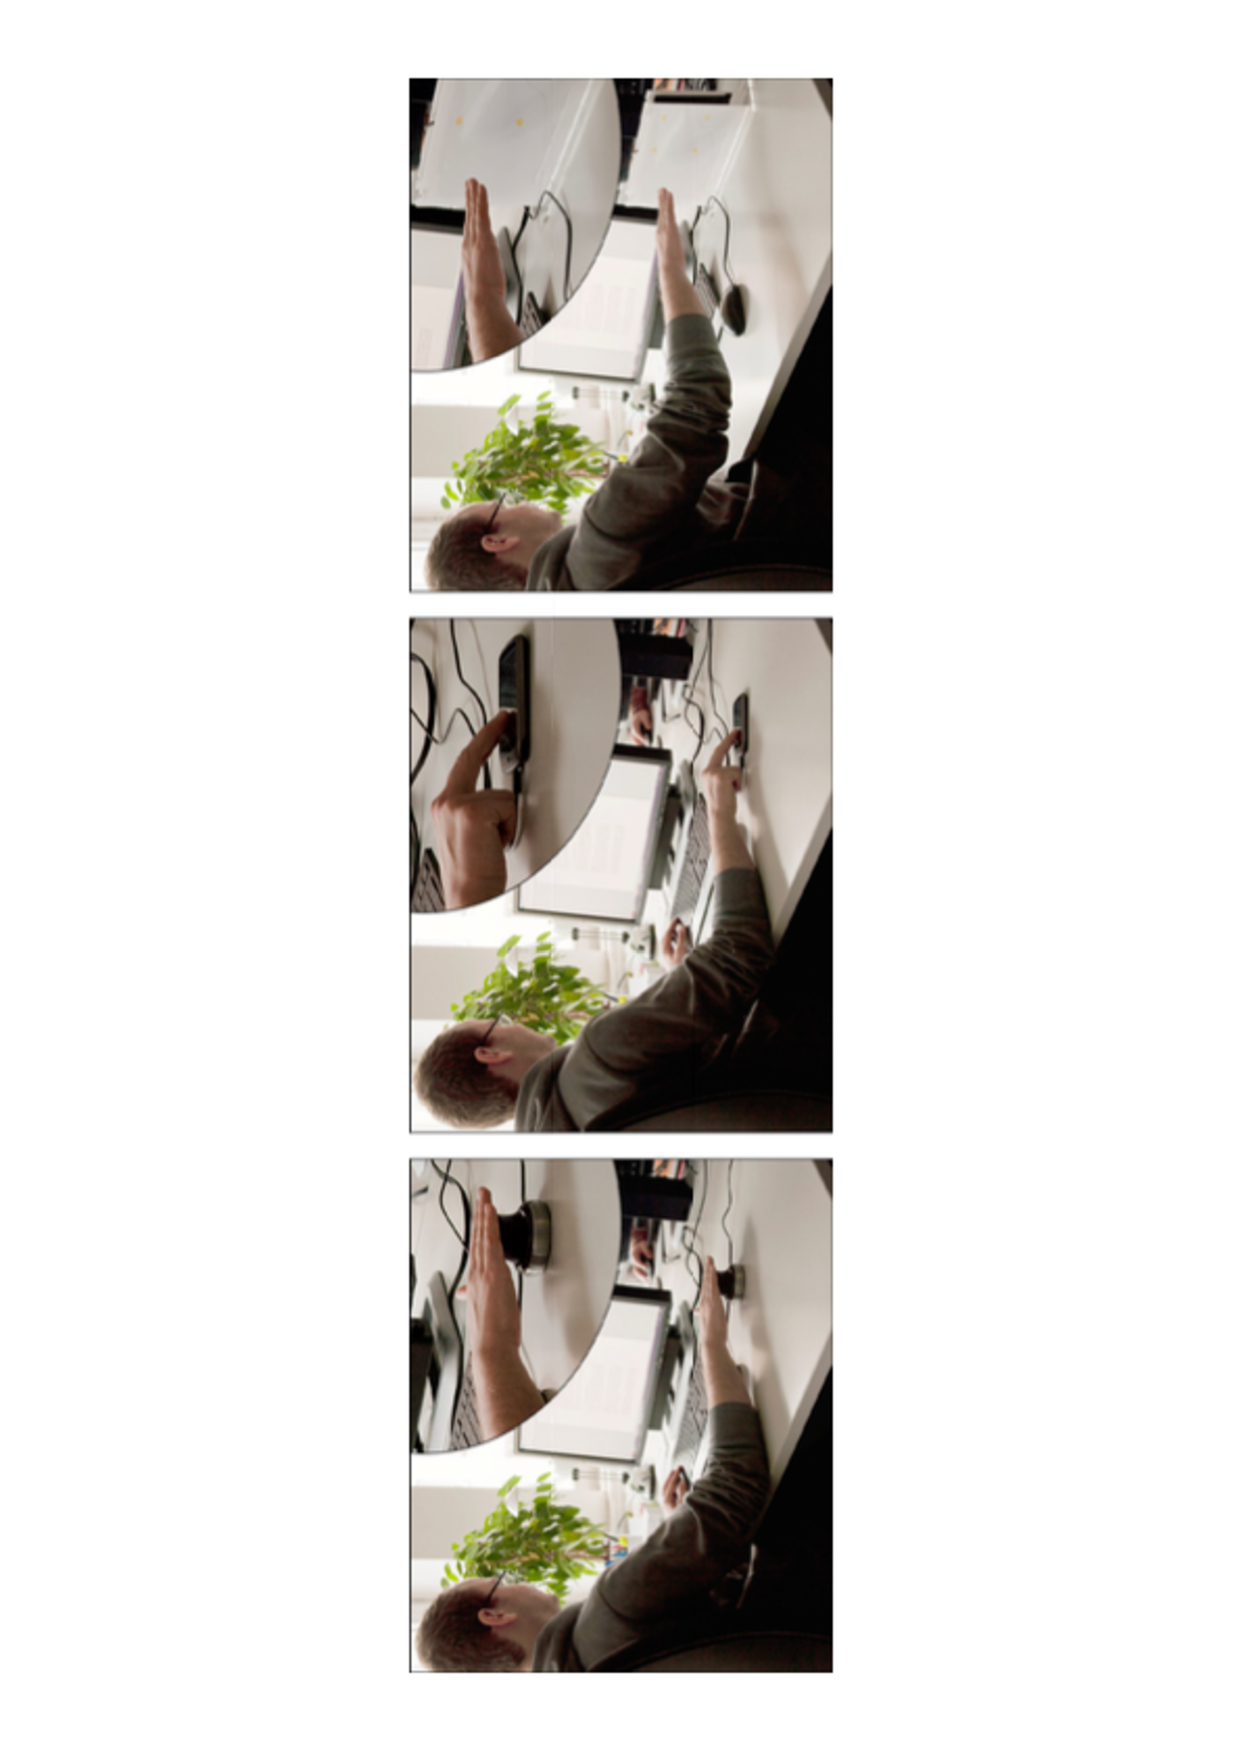
\includegraphics[resolution=300,width=0.70\textwidth]{InputModalitiesMusicControl}
	\caption{Illustration af de tre modaliteter, der bruges til perifer interaktion, fra venstre mod højre; knop-baseret håndtag, touchskærm og semaforisk gestik, \parencite[s. 163]{PDF:ComparingInputModalities}.}
	\label{fig:InputModalitiesMusicControl}
\end{figure}
\noindent
%
Herefter foretog \textcite[ss. 169-174]{PDF:ComparingInputModalities} en otte ugers feltundersøgelse, hvor testpersonerne brugte hver af de tre modaliteter igennem en to ugers periode samt tastaturets egne funktioner. For at undersøge om det er muligt at allokere interaktionen med musikafspilleren til den perifere opmærksomhed, målte \textcite[ss. 172-173]{PDF:ComparingInputModalities}, hvor mange gange testpersonerne interagerede med musikafspilleren, iTunes, uden at den var i fokus. Deraf fremgår det, baseret på testpersonernes bemærkninger, at de i højere grad var i stand til at udføre interaktionen, uden at rette fokus mod iTunes både ved det knop-baserede håndtag og dernæst touchskærmen, \parencite[ss. 172]{PDF:ComparingInputModalities}. Testpersonerne rangerede de semaforiske gestikker sidst, da de, ifølge \textcite[ss. 172-173]{PDF:ComparingInputModalities}, dels manglede den haptiske feedback og dels nød at overvære ændringerne i iTunes forårsaget af deres input, som føltes magiske. Sandsynligheden for at en interaktion med iTunes opstod, var størst ved de semaforiske gestikker, hvilket \textcite[s. 171]{PDF:ComparingInputModalities} pointerer kan skyldes registreringsproblemer. Sandsynligheden for at en interaktion opstod, var næststørst ved touchskærmen efterfulgt af det knop-baserede håndtag og den mindst sandsynlige interaktion var tastaturet. 

Derudover resulterede interaktionen med de tre modaliteter i en lavere mentalbelastning sammenlignet med tastaturet, \parencite[s. 172]{PDF:ComparingInputModalities}. Denne forskel i mentalbelastning kan fremme antallet af interaktioner, da testpersonerne generelt interagerede oftere med de tre modaliteter fremfor tastaturet, hvilket kan skyldes at tastaturet forårsagede en større mentalbelastning, \parencite[ss. 174-175]{PDF:ComparingInputModalities}.    

Ifølge \textcite[ss. 173-174]{PDF:ComparingInputModalities}, finder testpersonerne den nye interaktionsform, perifer interaktion, som værende et positivt tiltag, særligt fordi de kan kontrollere iTunes, uden at fjerne fokus fra den primære opgave. Endvidere forbinder testpersonerne semaforiske gestikker som værende futuristiske og sjove, \parencite[s. 174]{PDF:ComparingInputModalities}. I relation til semaforiske gestikker kommenterer \textcite[s. 177]{PDF:ComparingInputModalities}, at de egner sig til perifer interaktion og at de formegentlig i højere grad vil være at foretrække, såfremt de implementeres korrekt.\blankline
%                    
I undersøgelsen foretaget af \textcite{PDF:AStudyOnTheUseOfSemaphoricGestures} fokuseres der ligeledes på, om interaktionen med en musikafspiller kan foregå i den perifere opmærksomged og specifikt, hvordan det kan lade sig gøre via semaforiske gestikker. På baggrund af denne undersøgelse fremgår det, at testpersonerne foretrækker at interaktionen bygger på semaforiske gestikker fremfor at interaktionen skal foregå via tastaturet, hvilket gør sig særligt gældende, når tastaturet er uden for rækkevidde af den primære opgave, \parencite[s. 1963]{PDF:AStudyOnTheUseOfSemaphoricGestures}. Dog påpeger testpersonerne, at de oplevede udmattelse ved gentagne gange at udføre de semaforiske gestikker, \parencite[s. 1963]{PDF:AStudyOnTheUseOfSemaphoricGestures}. Ifølge \textcite[s. 1963]{PDF:AStudyOnTheUseOfSemaphoricGestures} vil det ikke nødvendigvis være tilfældet i den korrekte kontekst, da der højst sandsynligt ikke vil forekomme lige så mange interaktioner sammenlignet med det specifikke testscenarie. 

\textcite[s. 1964]{PDF:AStudyOnTheUseOfSemaphoricGestures} konkluderer, at der er signifikante fordele ved at anvende semaforiske gestikker, som interaktionsform i sekundære opgaver, og at restitutionstiden mellem udførelse af en sekundær opgave og den primære opgave mindskes sammenlignet med hvis interaktionen foregik via tastaturet.\blankline
%
Den sidste af de tre udvalgte undersøgelser, foretaget af \textcite[ss. 6-9]{PDF:AChairAsUbiquitousInputDevice}, fokuserer på, hvordan en interaktiv stol kan anvendes til perifer interaktion med en musikafspiller. De forskellige kommandoer, som testpersonerne kan udføre ved hjælp af den interaktive stol er repræsenteret på \autoref{fig:ChairGestures}. 
%
\begin{figure}[H]
	\centering
	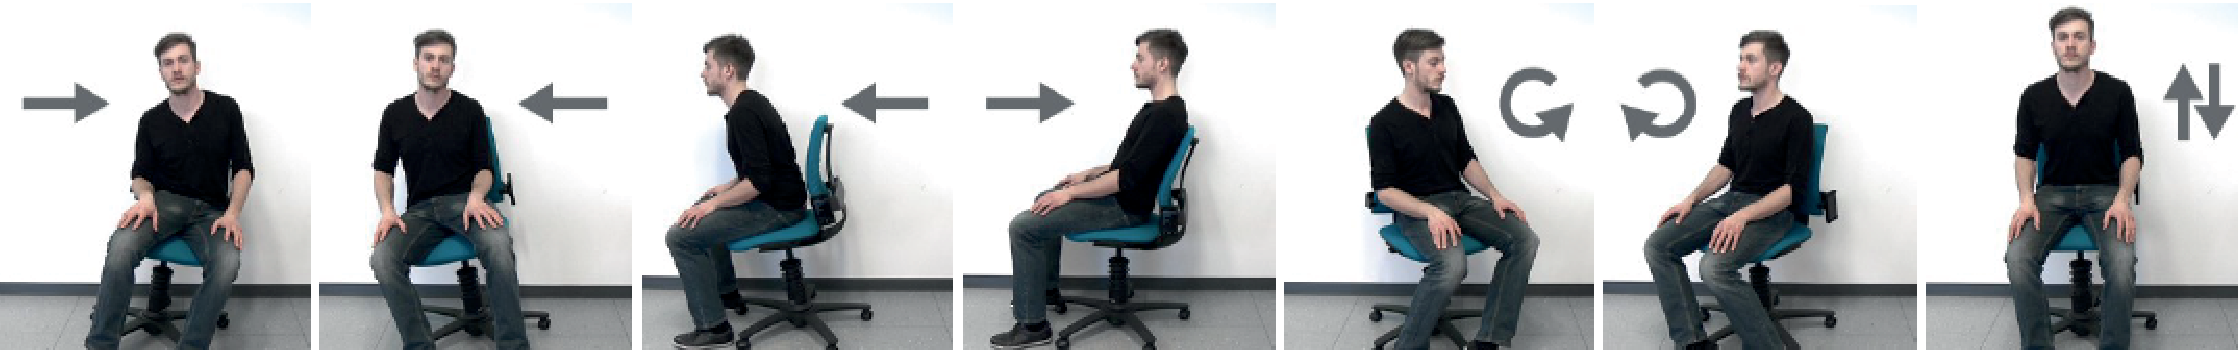
\includegraphics[resolution=300,width=0.70\textwidth]{ChairGestures}
	\caption{De syv forskellige kommandoer, som kan udføres via den interaktive stol, \parencite[s. 3]{PDF:AChairAsUbiquitousInputDevice}.}
	\label{fig:ChairGestures}
\end{figure}
\noindent
%
Selvom det tager testpersonerne længere tid at udføre selve interaktionen med den interaktive stol sammenlignet med tocuh og tastatur, så var responstiden kortest for den interaktive stol, \textcite[s. 7]{PDF:AChairAsUbiquitousInputDevice}. Responstid defineres som tiden fra at testpersonen modtager en notifikation om, at de skal interagere med musikafspilleren, til at testpersonen påbegynder sin interaktion, \parencite[s. 6]{PDF:AChairAsUbiquitousInputDevice}. Derudover målte \textcite[s. 7]{PDF:AChairAsUbiquitousInputDevice} restitutionstid, som var signifikant kortere for den interaktive stol. Restitutionstid defineres som den tid det tager testpersonerne, at vende tilbage til den primære opgave efter interaktionen med musikafspilleren. \textcite[s. 8]{PDF:AChairAsUbiquitousInputDevice} understreger vigtigheden af et pålideligt genkendelsessystem, da testpersonerne ikke får andet end funktionel feedback fra musikken, da der ellers kan opstå forvirring, hvis systemet ikke registrer gestikken. Ydermere understøtter denne undersøgelse, at semaforiske gestikker fordelagtigt kan anvendes til perifer interaktion for at reducere den mentalebelastning og stadig tillade brugeren at holde fokus på den primære opgave, \parencite[s. 8]{PDF:AChairAsUbiquitousInputDevice}. Semaforiske gestikker svarer i denne sammenhæng til, hvordan testpersonerne interagerer med den interaktive stol. \blankline
%
Det er vigtigt at pointere, at de relaterede undersøgelser ikke nødvendigvis gengiver interaktionen eller situationen, hvorved interaktionen opstår i relation til Bang $\&$ Olufsens produkt. Da det tyder på, at gestikker er at foretrække til perifer interaktion med en musikafspiller på computeren, antages det, at det samme er gældende for interaktion med et musikanlæg. 

Med udgangspunkt i de relaterede undersøgelser, der primært inkluderer semaforiske og manipulerende gestikker som interaktionsform, vil der i projektsammenhæng afgrænses til at undersøge disse to former i forbindelse med perifer interaktion.   
